\documentclass[../main.tex]{subfiles}
\begin{document}
\renewcommand{\baselinestretch}{1.5}

\chapter{High-level overview}
This chapter contains a high-level overview of the project, describing functional requirements, and an overview of tools and technologies that will be leveraged. This will be further expanded in the third chapter.

\section{Functional requirements}
The functional requirements are based on the user stories approach from Agile. The project is considered a success when the below stories are met:\\

\textbf{A user must be able to...}
\begin{itemize}
    \item Queue new request for a docker instance
    \item Cancel pending requests
    \item Insert external data into the container for processing
    \item Retrieve results after processing
\end{itemize}


\textbf{A admin must be able to...}
\begin{itemize}
    \item Monitor the status of the queue
    \item Monitor the status of the docker environment
    \item Identify the container's creator
\end{itemize}


\section{Design overview}
This section contains a brief overview of how the end result should look like, and a brief description of the tools and technologies leveraged.
\subsection{Design illustration}
Figure \ref{fig:high_level_design} illustrates how users can connect to the server through a web interface, and also get access to the shared storage through the server. The server will then take request and spread them across the worker nodes, and save the results on a shared storage medium for retrieval.
\begin{figure}[H]
    \centering
    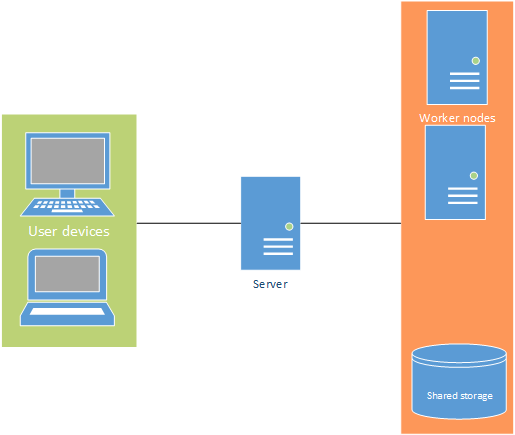
\includegraphics[scale=.6]{img/High_level_design.png}
    \caption{High-level overview of how devices will connect to the finished infrastructure}
    \label{fig:high_level_design}
\end{figure}

% egen side
\newpage
\subsection{Tools}
\begin{itemize}
    \item VIM\cite{vim} and Visual Studio Code\cite{vscode}\\These are the primarily used editors and IDE for the project
    \item Git\cite{git}\\ Is a version control system, that enables a group of developers to work together on the same project in an organized manner
    \item Bitbucket\cite{bitbucket}\\ Distributed version control system for usage with Git
    \item JIRA\cite{jira}\\ Issue tracker and time logger
    \item Vue.js devtools\cite{vuejsdevtools}\\Chrome and Firefox extension that enables developers to inspect and edit live Vue components
    \item Postman\cite{postman}\\ Allows developers to create custom requests to API and inspect the response
\end{itemize}

% egen side
\newpage
\subsection{Technologies}
\begin{itemize}
    \item Docker \cite{docker}\\ Docker is a tool to deploy and manage docker containers 
    \item Docker-compose \cite{dockercomp}\\ Docker-compose used for handling a multi docker environment.
    \item MySQL \cite{mysql}\\ MySQL is a relational database that allows persistent storage of queriable data
    \item Kubernetes \cite{kube}\\ Kubernetes is a container orchestrating tool
    \item Grafana \cite{grafana}\\Grafana is used to graph metric data from multiple data sources
    \item Prometheus \cite{prometheus}\\Prometheus is a time-series database
    \item Cadvisor \cite{cadvisor}\\Cadvisor gathers live information from docker containers
    \item Alertmanager \cite{alertmanager}\\Alertmanager is used to manage the alerts regarding the data
    \item Node aexporter \cite{nodeexporter}\\Nodeexporter collects host metrics
\end{itemize}

% egen side
\newpage
\subsection{Frameworks and libraries}
\begin{itemize}
    % \item Golang\cite{golang}\\ 
    \item py3nvml \cite{py3nvml}\\ A Python library used to gather information about NVIDIA Graphics Card
    \item Vue.js \cite{vuejs}\\ A framework to build full-fledged web applications in javascript
    \item Laravel/PHP \cite{laravel}\\ A framework to build PHP based web applications
\end{itemize}
\end{document}